\documentclass[9pt,lineno]{elife}
\usepackage[version=4]{mhchem}
\usepackage{siunitx}
\DeclareSIUnit\Molar{M}

\usepackage{amsmath}
\usepackage{gensymb}
\graphicspath{{images/}}
\usepackage{caption}
\usepackage{subcaption}


%%%%%%%%%%%%%%%%%%%%%%%%%%%%%%%%%%%%%%%%%%%%%%%%%%%%%%%%%%%%
%%% ARTICLE SETUP
%%%%%%%%%%%%%%%%%%%%%%%%%%%%%%%%%%%%%%%%%%%%%%%%%%%%%%%%%%%%
\title{Voltage to Calcium Transformation Improves Direction Selectivity in \textit{Drosophila} T4 neurons}

\author[1*]{Firstname Middlename Surname}
\author[1,2\authfn{1}\authfn{3}]{Firstname Middlename Familyname}
\author[2\authfn{1}\authfn{4}]{Firstname Initials Surname}
\author[2*]{Firstname Surname}
\affil[1]{Max Planck Institute of Neurobiology, Martinsried, Germany}

\corr{email1@example.com}{FMS}
\corr{email2@example.com}{FS}

\contrib[\authfn{1}]{These authors contributed equally to this work}
\contrib[\authfn{2}]{These authors also contributed equally to this work}

\presentadd[\authfn{3}]{Department, Institute, Country}
\presentadd[\authfn{4}]{Department, Institute, Country}

\usepackage[citestyle=authoryear-icomp,bibstyle=nature, ibidtracker=false,sorting=ynt]{biblatex}

\addbibresource{Reference.bib}

\begin{document}
\maketitle

\begin{abstract}
Analyzing how information is transmitted through neurons and synapses is crucial to understand how neural computation is carried out. A critical step in neural information processing is the transformation of voltage signals into calcium signals. However, the effect of voltage to calcium transformation on neural responses to different sensory stimuli is not well understood. Here, we use in vivo, two-photon imaging of genetically encoded voltage \& calcium indicators - Arclight and GCaMP6f respectively, to measure responses in \textit{Drosophila} direction-selective T4 neurons. Comparison between Arclight \& GCaMP6f signals revealed calcium signals to have much higher direction selectivity compared to voltage signals. Using these recordings we further build a model which transforms T4 voltage responses to calcium responses. The model reproduces calcium responses across different visual stimuli. These findings reveal that voltage to calcium transformation involving non-linearity \& low-pass filtering results in a higher direction selectivity in T4 cells.

%Fluorescence changes in response to changes in neuronal calcium level have been widely used to study neural activity. More studies using voltage imaging and electrophysiology are now being done to record neural responses in \textit{Drosophila} visual circuit. However, the effect of voltage to calcium transformation on neural responses to different sensory stimuli have not been well understood. Here, we use in vivo, two-photon imaging of genetically encoded voltage \& calcium indicators - Arclight and GCaMP6f respectively, to measure responses in \textit{Drosophila} T4 neurons. Comparison between Arclight \& GCaMP6f signals revealed calcium signals to have significantly higher direction selectivity compared to voltage signals. Using these recordings we further build a model which transforms T4 voltage responses to calcium responses. The model reproduces calcium responses across different visual stimuli. These findings reveal that voltage to calcium transformation involving non-linearity \& low-pass filtering results in a higher direction selectivity in T4 cells.

\end{abstract}

\section{Introduction}
In order to guide animal behavior, neurons perform a wide range of computations. Neurons encode information via dynamic changes in neuronal membrane potential and intracellular calcium concentration. Mostly, neurons communicate via chemical synapses which requires the release of neurotransmitters. When the presynaptic membrane is sufficiently depolarized, voltage-gated calcium channels open and allow $Ca^{2+}$ to enter the cell \parencite{Llinas1981}. Calcium entry leads to the fusion of synaptic vesicles with the membrane and release of neurotransmitter molecules into the synaptic cleft \parencite{Chapman2002}.  As neurotransmitters diffuse across synaptic cleft, they bind to receptors in the postsynaptic membrane, causing postsynaptic neuron to depolarize or hyperpolarize, and thus the information gets passed on from presynaptic to postsynaptic neuron \parencite{DiMaio2008}. Understanding voltage to calcium transformation in neurons is therefore crucial to understand neural information processing and neural computation. 

A classic example of neural computation can be found in how \textit{Drosophila} neurons compute the direction of visual motion \parencite{Borst2020}. In \textit{Drosophila} visual information is processed via parallel ON (contrast increments) and OFF (contrast decrements) pathways \parencite{Joesch2010, Eichner2011}. Direction selectivity emerges three synapses downstream of photoreceptors, in T4 and T5 for ON and OFF pathways respectively. Four subtypes of T4 and T5 cells exist, each responding selectively to one of the four cardinal directions \parencite{Maisak2013}. The underlying mechanisms generating direction selectivity and cellular correlates implementing these mechanisms have been studied extensively over the years. Classically two opposing models have been proposed for the computation of direction selectivity. Both these models use two input lines, where one of the input line has been asymmetrically delayed compared to other, which is then followed by a nonlinear interaction. The Hassenstein-Reichardt (HR) model, proposes a preferred direction enhancement (PDE) \parencite{Hassenstein1956}, while Barlow-Levick (BL) model proposes a null direction suppression (NDS) \parencite{Barlow1965}. 

Two major experimental approaches have been used to record signals from T4 \& T5 neurons. One approach has been to use changes in intracellular calcium concentration as an indicator for neural activity and the other has been to record changes in membrane potential as a proxy for neural activity. Studies in T4 \& T5 using calcium imaging have provided functional evidence for PDE \parencite{Fisher2015, Salazar-Gatzimas2016} and combination of both PDE \& NDS \parencite{Haag2016, Leong2016, Haag2017}. In contrast, \cite{Gruntman2018} using whole-cell patch clamp recording in T4 cells found NDS only. A study in T5 using voltage imaging of ASAP2f \parencite{Wienecke2018} found neither PDE nor NDS. A recent study using whole-cell patch clamp recordings \parencite{Groschner2022} has provided evidence for biophysical implementation of multiplication-like nonlinear operations in T4 neurons. This difference in findings between voltage and calcium studies requires further investigation of voltage to calcium transformation in T4 \& T5 neurons.

Electrophysiology has been the most frequently used method to measure the membrane potential changes in neurons. However, due to the small size of neurons in the optic lobe, single-cell electrophysiological recordings of these neurons have been difficult. Genetically encoded voltage indicators (GEVIs) have evolved as powerful tools for recording changes in neuronal membrane potentials. Optical methods of monitoring brain activity are appealing because they allow simultaneous, noninvasive monitoring of activity in many individual neurons. We used a fluorescence protein (FP) voltage sensor called Arclight \parencite{Jin2012}. Arclight is based on the fusion of voltage sensing domain of \textit{Ciona intestinalis} voltage sensitive phosphatase \parencite{Murata2005} and the fluorescent protein super ecliptic pHluorin with an A227D mutation. Arclight's fluorescence decreases with membrane depolarization and increases with membrane hyperpolarization. Arclight has been shown to robustly report both subthreshold events and action potentials in genetically targeted neurons in the intact \textit{Drosophila} brain \parencite{Cao2013}. Here, we used in-vivo two photon imaging of GCaMP6f \parencite{Chen2013} \& Arclight to record changes in intracellular calcium concentration and changes in membrane potential respectively.

\section{Results}

We used a driver line to express genetically encoded calcium indicator GCaMP6f \parencite{Chen2013} in T4 cells projecting to layer3 of lobula plate, and hence having upward motion as their Preferred Direction (PD) and downward motion as their Null Direction (ND). We then used the same driver line to express genetically encoded voltage indicator Arclight \parencite{Jin2012}. %Arclight decreases its fluorescence in response to depolarisation and increases in response to hyperpolarization.
In order to compare the voltage and calcium signals, we used the same set of stimuli, while recording the neural activity in T4c cells dendrites in medulla layer 10 using 2-photon microscopy \parencite{Denk1990}. The complete stimuli set included square-wave gratings and ON edges moving in different directions at varying speeds and contrasts.

Figure \ref{PDNDspeed}A shows the change in fluorescence for Arclight (black) and GCaMP (red) in response to gratings moving at 4 different speeds and 2 different directions (upper row PD, lower row ND). As the grating stimuli consists of alternate bright and dark bars moving in a certain direction, we see a modulation in the Arclight and GCaMP responses to it. The modulation in GCaMP responses was seen only for slower speeds, while Arclight responses had modulation even for faster speeds. The magnitude of response was much higher for GCaMP ($\approx2.0 \Delta F/F$) compared to Arclight ($\approx -0.06 \Delta F/F$). The peak responses (maximum $\Delta F/F$) decreased with increase in stimuli speed both for GCaMP and Arclight (figure \ref{PDNDspeed}B). To understand if voltage to calcium transformation affects direction selectivity in T4 cells, we compared its responses to gratings moving in PD and ND. GCaMP responses in ND were negligible compared to its responses in PD, while for Arclight responses in ND were considerable compared to its responses in PD. We quantified the direction selectivity using a Direction Selectivity Index (DSI) calculated as the difference of the peak responses to preferred and null direction, divided by the sum of the peak responses. The results reveal a high degree of direction selectivity of close to 1 for GCaMP for slower velocities, compared to low degree of direction selectivity ($\approx0.4$) for Arclight (figure \ref{PDNDspeed}E).

In a second set of experiments, we used a bright edge moving at 4 different velocities in PD or ND on a dark background. Figure \ref{PDNDspeed}C shows Arclight (black) \& GCaMP (red) responses to these moving edges. As the edge moves from bottom to top of the stimulus arena, it hits the receptive field of T4c neurons ($\approx15\degree$) only once and there is only a single peak in the response, not a modulation as there was with gratings. The peak response decreased with increase in stimuli speed for GCaMP, while the peak response remained almost constant for Arclight throughout all speeds (figure \ref{PDNDspeed}D). Similar to grating responses when comparing edge responses in PD \& ND, GCaMP had negligible response in ND while Arclight had considerable responses in ND compared to responses in PD. The direction selectivity index was again much higher for GCaMP compared to Arclight (figure \ref{PDNDspeed}F). These results together show GCaMP signals to have high level of direction selectivity compared to Arclight signals both for grating and edge stimuli.

Spatial contrast i.e. the difference between adjacent luminance values, provides information about objects, textures, and motion and is important for diverse visual processes. We were therefore interested in comparing voltage and calcium signal for different contrast conditions since contrast computation is essential to visual perception. We varied the stimulus strength by varying the contrast i.e. brightness difference between bright and dark bars for grating, and between moving edge and background for edge stimuli. Figure \ref{PDNDcontrast}A shows Arclight (black) \& GCaMP (red) responses to gratings moving at 30 deg/s at 4 different contrasts. Increasing contrast increases stimulus strength, resulting in an increase in response for both Arclight and GCaMP. As discussed earlier, we observe a modulation in the T4c response to gratings caused by alternate bright and dark bars. GCaMP responses however is not only modulated, but also rises steadily over time. This is interesting particularly because we do not see such a rise for Arclight responses. For Arclight responses we have only the modulation, whereas for GCaMP responses we have both the modulation and slow rise over time. Figure \ref{PDNDcontrast}C shows Arclight \& GCaMP responses to ON edge moving at the same speed at 4 different contrasts. The peak response (maximum $\Delta F/F$) increased with increase in contrast (figure \ref{PDNDcontrast}D). Similar to previous experiments, the direction selectivity index was much higher for GCaMP ($\approx1.0$) compared to that for Arclight ($\approx0.04$) (figure \ref{PDNDcontrast}E,F). 

In the results presented so far we compared responses for two directions - PD and ND. We next asked how does the comparison look if instead of two directions, responses for 12 directions are taken into account. In figure \ref{DirTuning}A, B we plot T4c Arclight \& GCaMP normalized peak responses for gratings moving in 12 directions at 4 different speeds and contrasts respectively. The directional tuning is much sharper for GCaMP compared to Arclight. To quantify this we calculated the directional tuning index $L_{dir}$ \parencite{Mazurek2014} for each speed and contrast stimuli condition. We calculate the index as a vector sum of the peak responses and divide the magnitude of the resultant vector by the sum of individual vector magnitudes. The directional tuning index for slower speeds and all contrasts was much higher for GCaMP ($\approx0.7$) compared to that of Arclight ($\approx0.2$). These results together show GCaMP to have a higher degree of directional tuning across different speeds and contrasts compared to Arclight.

How does the voltage to calcium transformation leads to calcium signals with significantly higher direction selectivity and tuning compared to voltage signals ? To address this question, we constructed an algorithmic model (figure \ref{Modelillustration}) which takes Arclight signals as inputs and outputs GCaMP signal. In order to find the optimal parameter values, we first define an error function. The error is calculated as $\text{(Model data - Experiment data)}^2 / \text{(Experiment data)}^2$. The model takes as input Arclight data across all stimuli conditions - grating speed(48), grating contrast(48), edge speed(8), edge contrast(8) i.e. a total of 112 different stimuli conditions. Next, the model produces output and totals the error for all stimuli conditions. Then, we use Python SciPy optimize minimize function to find the optimal parameters values of the model that correspond to the minimum error.

We started with a simple model (figure \ref{Modelillustration}A). The model first passes the Arclight signal through a high-pass filter. The high-pass filter would bring input Arclight signal closer to actual voltage signal by removing Arclight indicator dynamics. This is followed by a threshold since voltage changes below a certain threshold would not affect the calcium level in the cell. Now, few experimental observations which we took into consideration for building up the model further were as follows : First, the GCaMP response to grating had modulation only for slower speeds, whereas Arclight showed modulations even at faster speeds(figure \ref{PDNDspeed}A). This indicates towards GCaMP signal being a low-pass filtered version of the Arclight signal. In the simple model, we used a single low-pass filter followed by a gain and time-shift. Multiplication with a gain factor is required since GCaMP signals have a much higher magnitude compared to Arclight. The time-shift aligns the model signal with the calcium signal. However, the simple model with single low-pass filter could not reproduce responses across all stimuli. The total error for complete dataset fit for the simple model was around $34\%$. Specifically, the simple model fails to reproduce the edge responses. Second, the GCaMP responses in addition to modulation also had a steady rise over time whereas Arclight signal only had modulation (figure \ref{PDNDspeed}A, \ref{PDNDcontrast}A). For producing the edge responses and modulation in gratings responses, the model needs a low-pass filter with a smaller time constant. However to simulate the steady rise in the gratings signal the model needs a low-pass filter with a larger time constant. Hence, we combined the output of two low-pass filters. Combining the low-pass filters output with an addition (figure \ref{Modelillustration}B) did not lead to much improvement with error being around $37\%$ for complete dataset fit. However, combing both the outputs with a multiplication led to signifciant decrease in the error. The error for the multiplicative model (figure \ref{Modelillustration}C) was around $14\%$. 

The multiplicative model thus has in total 6 parameters - high-pass filter time constant, threshold, low-pass filter 1 time constant, low-pass filter 2 time constant, gain and shift.  The multiplicative model was able to reproduce calcium signals across different visual stimuli (figure \ref{PDNDModel}). The model could produce both the modulation and slow rise in the GCaMP signal in response to grating (figure \ref{PDNDModel} A). The model could also reproduce the ON edge speed tuning responses across different speeds (figure \ref{PDNDModel} C,D). The directional tuning index $L_{dir}$ also were similar for model and experimental data across slower speeds and all contrasts (figure \ref{PDNDModel} E,F). Thus the model is able to successfully reproduce experimental calcium data across different stimuli.  

The slow rise in GCaMP signals over time is due to the properties of T4 cells or due to the properties of GCaMP6f. To answer this we used a faster indicator GCaMP8f \parencite{Zhang2020}. GCaMP8f was expressed in T4c cells using the same driver line. The experiments were repeated using gratings stimuli in 12 directions at 4 speeds and ON edge in PD and ND. T4c cells GCaMP8f responses were similar to GCaMP6f responses. The modulation and slow rise of the signal could still be seen (Supplement figure). This shows that slow rise in calcium signal is indeed due to T4 cells intrinsic properties and not due to slowness of GCaMP6f indicator. We further compared the model parameters values for GCaMP6f data fit and GCaMP8f data fit (figure \ref{gcampcomparison}). The model parameters had similar values with time constants having slightly smaller values for GCAMP8f as it is a faster indicator.

     


\begin{figure}
\begin{fullwidth}
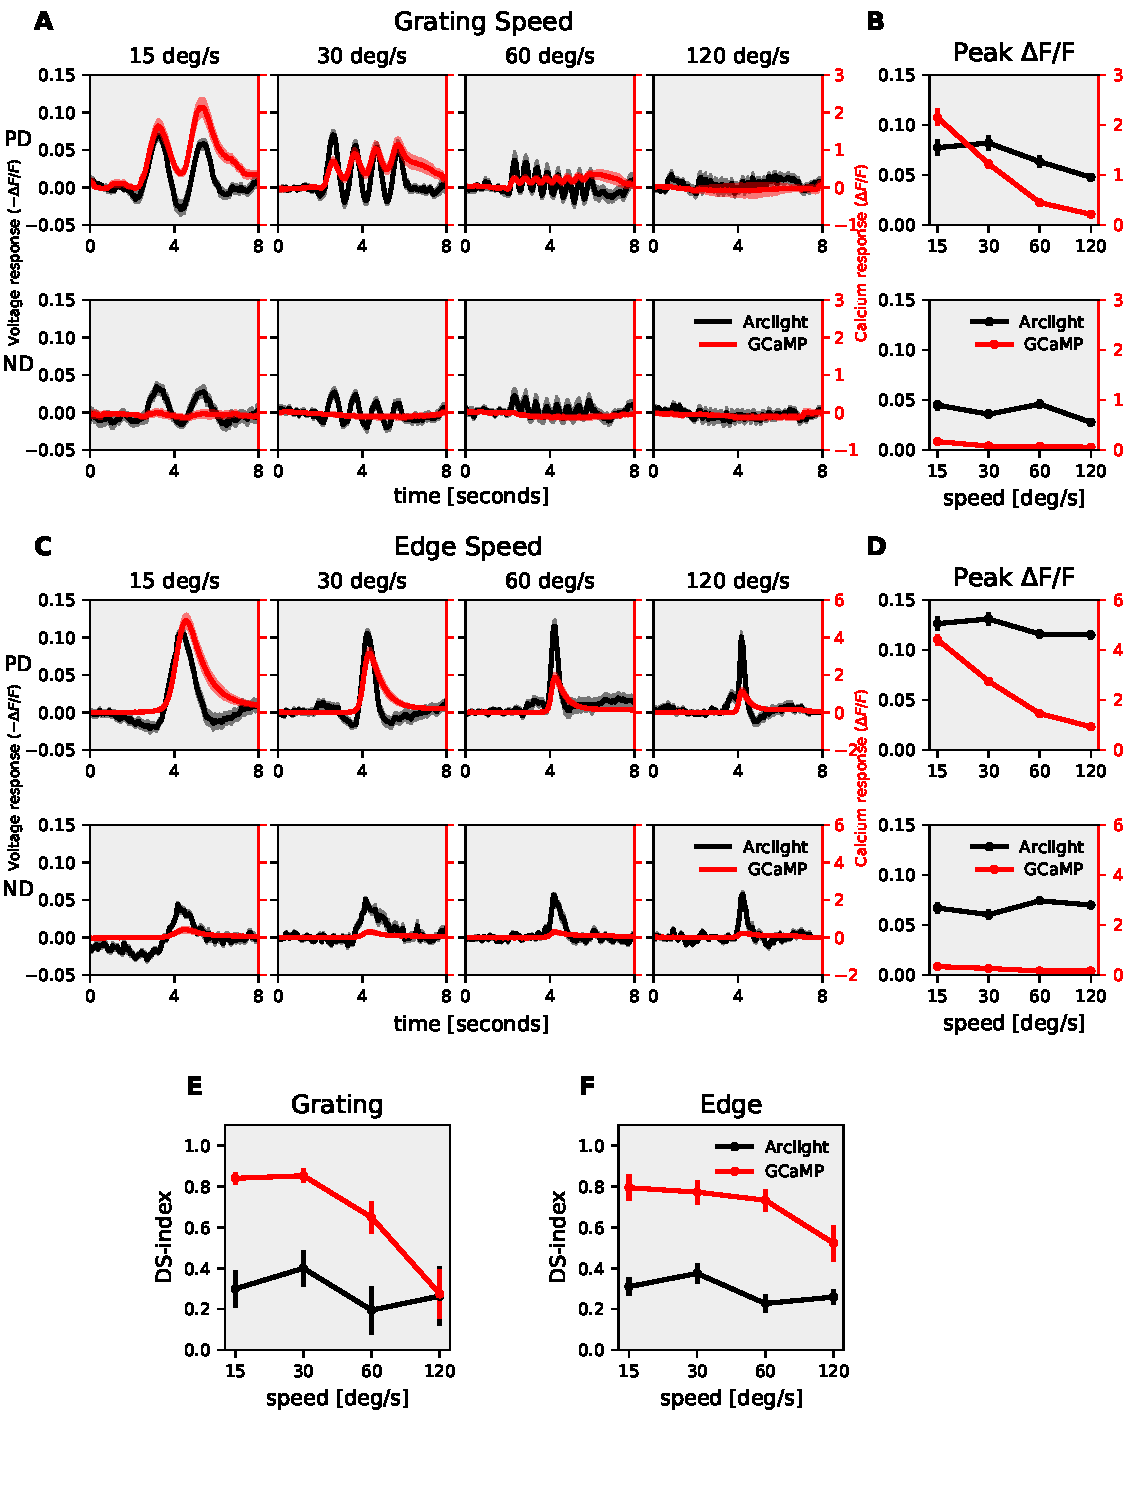
\includegraphics[width=0.84\linewidth]{figure1}
	%\includegraphics[height = 8cm]{Mi1_Medulla_GtACR}
\caption{\textbf{T4c voltage \& calcium speed tuning} : (A) T4c Arclight (black) \& GCaMP (red) responses to grating moving in PD (top row) \& ND (bottom row) at 4 different speeds. Data shows the mean $\pm$ SEM of T4c cell responses measured in 5 different flies. The plots have twin y-axis. The left y-axis of the plot represents Voltage responses i.e. changes in Arclight fluorescence ($-\Delta F/F$) and the right y-axis of the plot represents Calcium responses i.e. changes in GCaMP fluorescence ($\Delta F/F$) (B) T4c peak responses to grating moving in PD(top) \& ND(bottom) at 4 different speeds. (C) T4c Arclight (black) \& GCaMP (red) responses to ON-edge moving in PD (top row)\& ND (bottom row) at 4 different speeds. Data shows the mean $\pm$ SEM of T4c cell responses measured in 5 different flies. (D) T4c peak responses to ON-edge moving in PD \& ND at 4 different speeds. (E) Direction Selectivity Index (DSI) calculated as difference of peak responses in PD and ND divided by the sum of peak responses for grating (F) Direction Selectivity Index (DSI) for ON-edge.}

\label{PDNDspeed}
	
\end{fullwidth}
\end{figure} 

\begin{figure}
\begin{fullwidth}
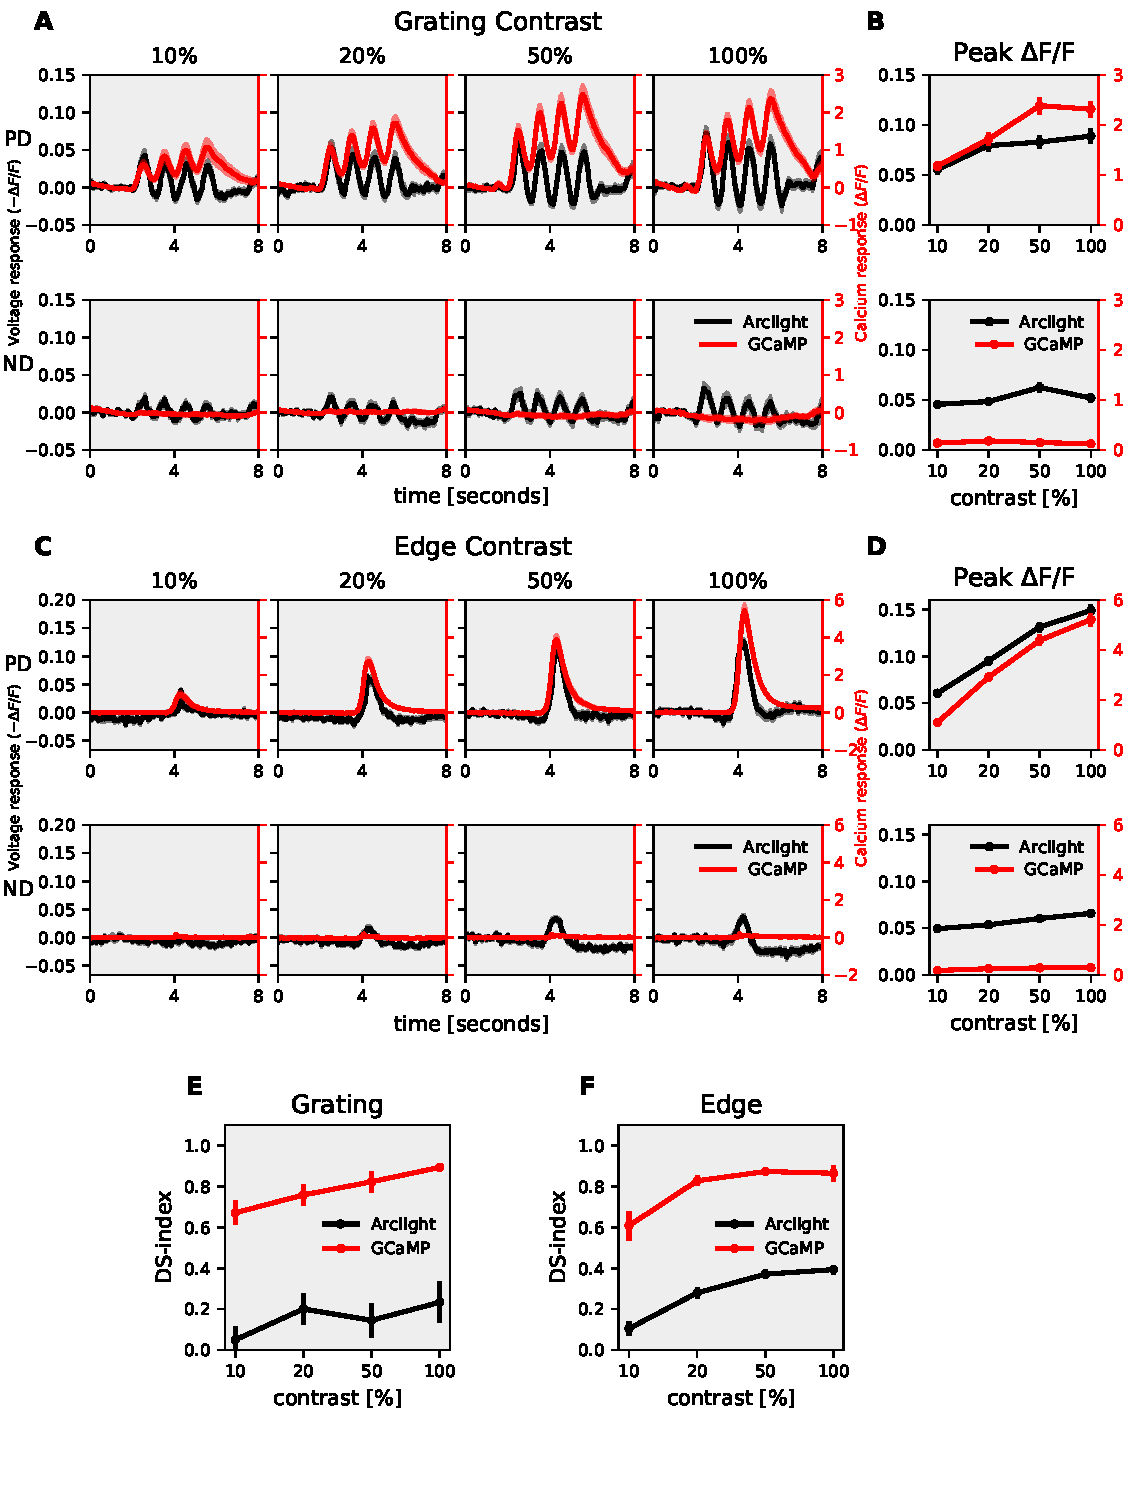
\includegraphics[width=0.84\linewidth]{figure2}
	%\includegraphics[height = 8cm]{Mi1_Medulla_GtACR}
\caption{\textbf{T4c voltage \& calcium contrast tuning} : (A) T4c Arclight (black) \& GCaMP (red) responses to grating moving in PD (top row) \& ND (bottom row) at 4 contrasts. Data shows the mean $\pm$ SEM of T4c cell responses measured in 5 different flies. The plots have twin y-axis. The left y-axis of the plot represents Voltage responses i.e. changes in Arclight fluorescence ($-\Delta F/F$) and the right y-axis of the plot represents Calcium responses i.e. changes in GCaMP fluorescence ($\Delta F/F$) (B) T4c peak responses to grating moving in PD(top) \& ND(bottom) at 4 different contrasts. (C) T4c Arclight (black) \& GCaMP (red) responses to ON-edge moving in PD (top row)\& ND (bottom row) at 4 different contrasts. Data shows the mean $\pm$ SEM of T4c cell responses measured in 5 different flies. (D) T4c peak responses to ON-edge moving in PD \& ND at 4 different contrasts. (E) Direction Selectivity Index (DSI) calculated as difference of peak responses in PD and ND divided by the sum of peak responses for grating (F) Direction Selectivity Index (DSI) for ON-edge.}

\label{PDNDcontrast}
	
\end{fullwidth}
\end{figure} 

\begin{figure}
\begin{fullwidth}
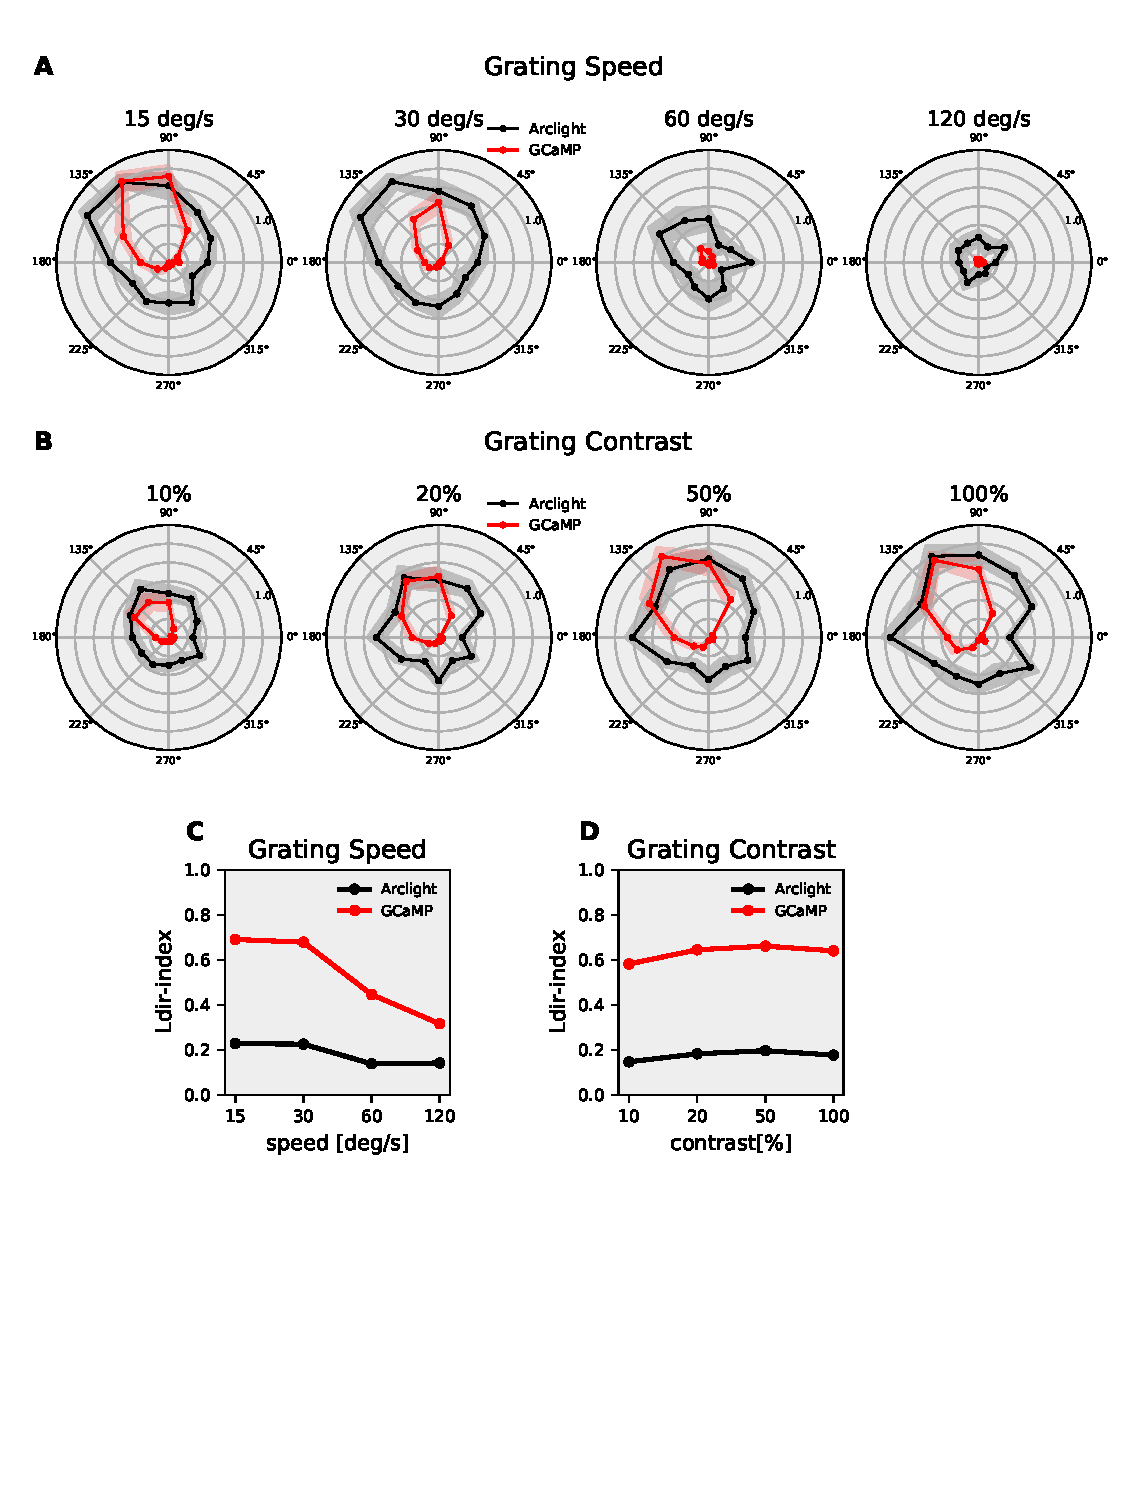
\includegraphics[width=0.84\linewidth]{figure3}
	%\includegraphics[height = 8cm]{Mi1_Medulla_GtACR}
\caption{\textbf{T4c voltage \& calcium direction tuning} : (A) T4c Arclight (black) \& GCaMP (red) normalized peak responses to grating moving in 12 directions at 4 speeds. Data shows the normalized mean $\pm$ SEM of T4c cell peak responses measured in 5 different flies. (B) T4c Arclight (black) \& GCaMP (red) normalized peak responses to grating moving in 12 directions at 4 contrasts. Data shows the normalized mean $\pm$ SEM of T4c cell peak responses measured in 5 different flies (C) The Directional Tuning Index $L_{dir}$ for grating moving at 4 different speeds. The Directional Tuning Index is calculated as a vector summation of the peak responses and the magnitude of resultant vector is divided by the summation of individual vector magnitudes. (D) The directional tuning index for grating at 4 different contrasts.}

\label{DirTuning}
	
\end{fullwidth}
\end{figure} 

\begin{figure}
\begin{fullwidth}
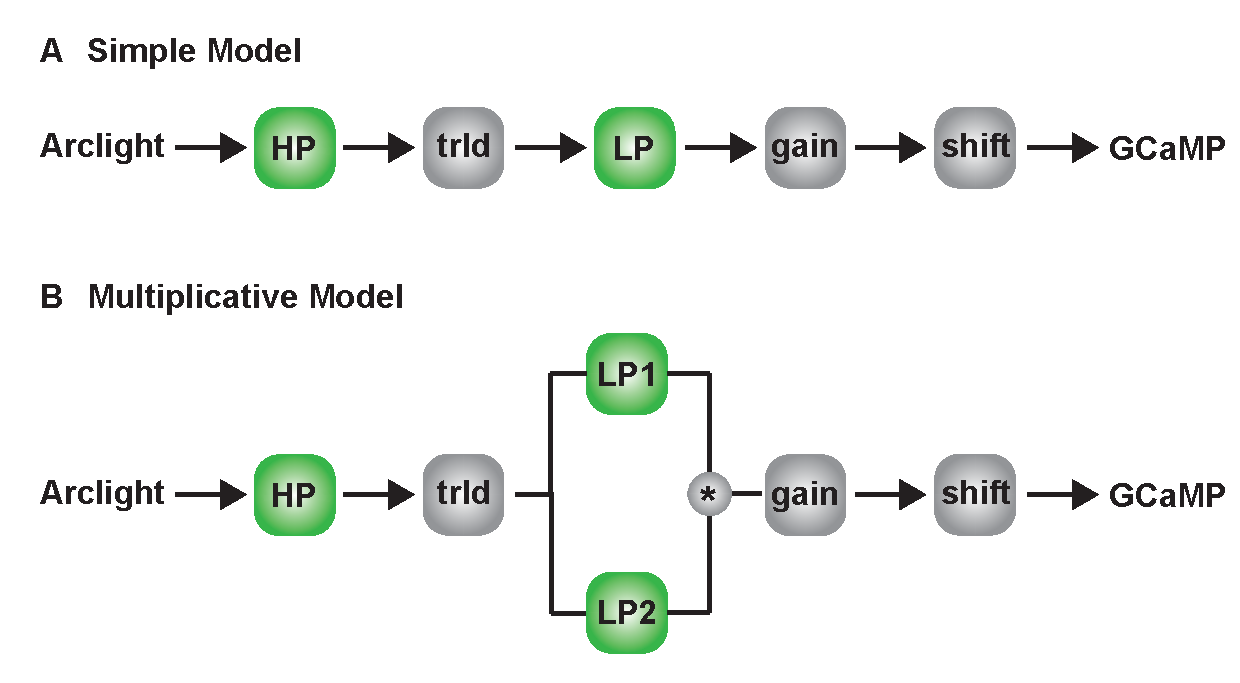
\includegraphics[width=0.84\linewidth]{figure4}
	%\includegraphics[height = 8cm]{Mi1_Medulla_GtACR}
\caption{\textbf{Models for producing GCaMP responses} : (A) Simple model consisting of High-Pass filter (HP), threshold(trld), Low-Pass filter(LP), gain and shift. (B) Additive model combining output of two low-pass filters via addition. (C) Multiplicative model combining output of two low-pass filters via multiplication. }

\label{Modelillustration}
	
\end{fullwidth}
\end{figure} 

\begin{figure}
\begin{fullwidth}
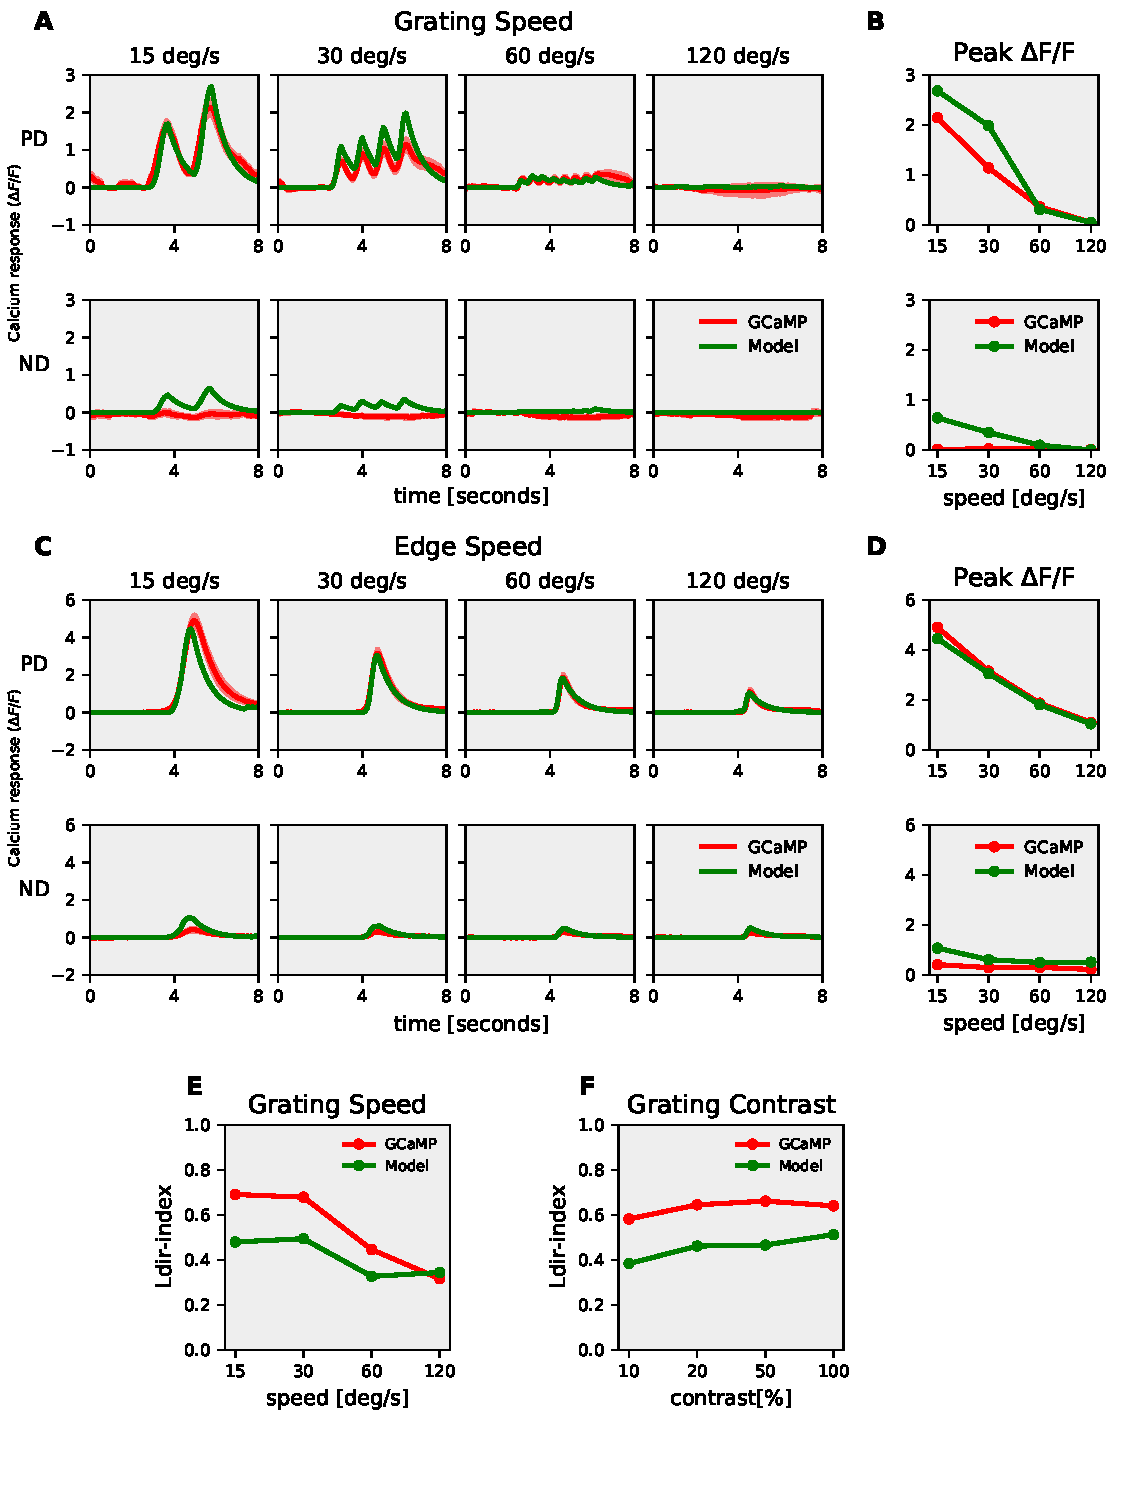
\includegraphics[width=0.84\linewidth]{figure5}
	%\includegraphics[height = 8cm]{Mi1_Medulla_GtACR}
\caption{\textbf{The Multiplicative model responses} : (A) T4c GCaMP (red) \& Multiplicative model (green) responses to grating moving in PD (top row) \& ND (bottom row) at 4 different speeds. (B) T4c GCaMP \& model peak responses to grating moving in PD(top) \& ND(bottom) at 4 different speeds. (C) T4c GCaMP (red) \& Multiplicative model (green) responses to ON-edge moving in PD (top row) \& ND (bottom row) at 4 different speeds. (D) T4c GCaMP \& model peak responses to ON-edge moving in PD(top) \& ND(bottom) at 4 different speeds. (E) The Directional Tuning Index $L_{dir}$ for GCaMP \& model for grating moving in 12 directions at 4 different speeds. (F) The Directional Tuning Index $L_{dir}$ for GCaMP \& model for grating moving in 12 directions at 4 different contrasts.}

\label{PDNDModel}
	
\end{fullwidth}
\end{figure} 

\begin{figure}
\begin{fullwidth}
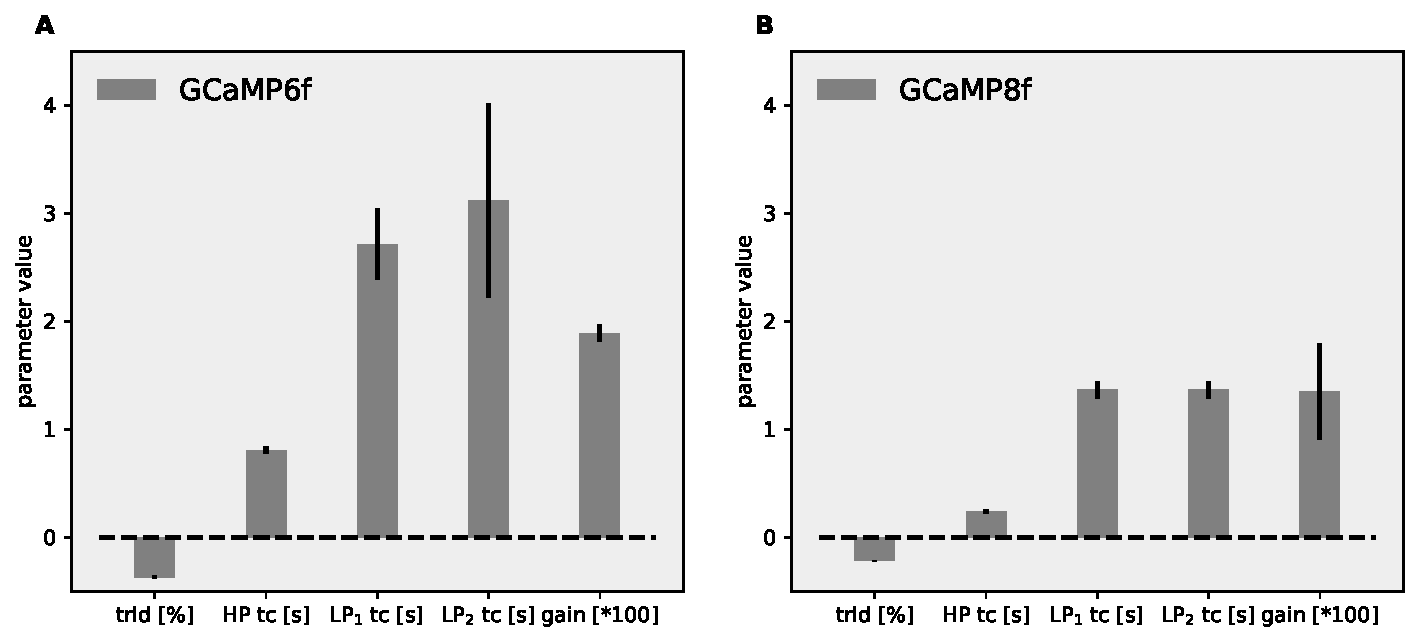
\includegraphics[width=0.84\linewidth]{figure6}
	%\includegraphics[height = 8cm]{Mi1_Medulla_GtACR}
\caption{\textbf{Model parameters comparison for GCaMP6f \& GCaMP8f} : Data shows mean $\pm$ SD for optimal parameters for the Multiplicative model. The data were fit for grating moving in 12 directions and 4 speeds, and for ON-edge moving in PD \& ND at 4 speeds.}

\label{gcampcomparison}
	
\end{fullwidth}
\end{figure} 




\section{Materials and Methods}
\subsection{Flies}
Flies (\textit{Drosophila melanogaster}) were raised at $25\degree C$ and $60\%$ humidity on a $12$ hour light/$12$ hour dark cycle on standard cornmeal agar medium. For calcium imaging experiments, genetically-encoded calcium indicator GCaMP6f \parencite{Chen2013} was expressed in T4 neurons with axon terminals predominantly in  layer 3 of the lobula plate. Similarly for voltage imaging experiments, genetically-encoded voltage indicator Arclight \parencite{Jin2012} was expressed in T4 layer 3 neurons. The flies genotype are as follows : 
\begin{enumerate}
\item w+ ; VT15785-Gal4AD / UAS-GCaMP6f; VT50384-Gal4DBD / UAS-GCaMP6f 
\item w+ ; VT15785-Gal4AD / UAS-Arclight; VT50384-Gal4DBD / + 
\end{enumerate}

\subsection{Calcium \& voltage imaging}
For imaging experiments, fly surgeries were performed as previously described \parencite{Maisak2013}. Briefly, flies were anaesthetized with CO$_2$ or on ice, fixed with their backs, legs and wings to a Plexiglas holder with back of the head exposed to a recording chamber filled with fly external solution. The cuticula at the back of the head on one side of the brain was cut away with a fine hypodermic needle and removed together with air sacks covering the underlying optic lobe. The neuronal activity was then measured from optic lobe on a custom-built 2-photon microscope as previously described \parencite{Maisak2013}. Images were acquired at 64 x 64 pixels resolution and frame rate 13 Hz with the Scanimage software in Matlab  \parencite{Pologruto2003}.

\subsection{Visual stimulation}
For the study of visual responses of T4c cells, visual stimuli were presented on a custom-built projector-based arena as described in \parencite{Arenz2017}. In brief : Two micro-projectors (TI DLP Lightcrafter 3000) were used to project stimuli onto the back of an opaque cylindrical screen covering $180\degree$ in azimuth and $105\degree$ in elevation of the fly's visual field. To increase the refresh rate from 60 Hz to 180 Hz (at 8 bit color depth), projectors were programmed to use only green LED (OSRAM L CG H9RN) which emits light between 500 nm to 600 nm wavelength. Two long-pass filters (Thorlabs FEL0550 and FGL550) were placed in front of each projector to restrict the stimulus light to wavelengths above 550 nm. This prevents overlap between GCaMP signal and arena light spectra. To allow only GCaMP emission spectrum to be detected, a band-pass filter (Brightline 520/35) was placed in-front of the photomultiplier. For all stimuli used here, we set the medium brightness to a 8-bit grayscale value of 50, which corresponds to a medium luminance of $55 \pm 11 cd/m^2$. Stimuli were rendered using custom written software in Python 2.7. 

\subsubsection{Stimuli}
Stimuli were presented with 3-5 repetitions per experiment in a randomized fashion. To measure the directional and speed tuning, square-wave gratings with a spatial wavelength of $30\degree$ spanning the full extent of the stimulus arena were used. The gratings were moved in 12 different directions from $0\degree - 360\degree$ at 4 different speed ($15degree/second - 120degree/second$). Similarly, to measure direction and contrast tuning, square-wave gratings with a spatial wavelength of $30\degree$ spanning the full extent of the stimulus arena were used. The gratings moved at a speed of $30degree/second$ in 12 different directions at 4 different contrast ($10\% - 100\%$). Edge responses were measured using ON edge i.e. bright edge moving on a dark background with full contrast. The ON edge moved in preferred direction (upward) or null direction (downward) at 4 different speed ($15degree/second - 120degree/second$).

\subsection{Data analysis}
Data analysis was performed using custom-written routines in Matlab and Python 2.7, 3.7. Images were automatically registered using horizontal and vertical translations to correct for the movement of brain. Fluorescence changes $(\Delta F/F)$ were then calculated using a standard baseline algorithm \parencite{Jia2010}. Regions of interest (ROIs) were drawn on the average raw image manually by hand in the medulla layer M10 for signals from T4 dendrites. Averaging the fluorescence change over this ROI in space resulted in a $(\Delta F/F)$ time course. Voltage imaging with Arclight and Calcium imaging with GCaMP were performed and analysed using same settings.

\printbibliography[heading=bibintoc]
\end{document}